\documentclass[answers,12pt,addpoints]{exam}
\usepackage{import}

\import{C:/Users/prana/OneDrive/Desktop/MathNotes}{style.tex}

% Header
\newcommand{\name}{Pranav Tikkawar}
\newcommand{\course}{01:640:481}
\newcommand{\assignment}{Final Exam Notes}
\author{\name}
\title{\course \ - \assignment}

\begin{document}
\maketitle
\tableofcontents

\newpage
\section*{Content}
\textbf{Exam 1}
\begin{itemize}
    \item 6.3 (Gamma Distribution)
    \item 8.1 (Sampling Distributions)
    \item 8.2 (Sample Mean)
    \item 8.4 (Chi-Squared Distribution)
    \item 8.7 (Order Statistics)
    \item 10.1 (Point Estimation)
    \item 10.2 (Unbiased Estimation)
    \item 10.8 (Maximum Likelihood Estimation)
\end{itemize}
\textbf{Exam 2}
\begin{itemize}
    \item 10.2 (unbiased)
    \item 10.3 (efficiency/Cramer Rao)
    \item 10.7 (Method of moments)
    \item 11.1 (Interval estimation)
    \item 11.2 (Estimation of Means)
    \item 11.3 (Estimation of Difference of Means)
    \item 11.6 (Estimation of Variance)
    \item 11.7 (Estimation of Ratio of Variance)
    \item 12.1 (Hypothesis Testing)
    \item 12.2 (Testing a Statistic Hypothesis)
    \item 7.3 \& 7.4 (Transformation theorem)
    \item 8.5 (t-distribution)
    \item 8.6 (f-distribution)
\end{itemize}
\textbf{Final}
\begin{itemize}
    \item 12.4 (Neyman-Pearson Lemma)
    \item 12.6 (Likelihood Ratio Test) 
    \item 13.1 (Tests of Hypothesis)
    \item 13.2 (Tests Concerning Means)
    \item 13.3 (Tests Difference of Means)
    \item 13.4 (Tests Concerning Variance)
\end{itemize}

\section*{Notes}
\subsection{Neyman-Pearson Lemma}
\begin{definition}[Power of a Test]
    The power of a test is the probability that the test rejects the null hypothesis when the alternative hypothesis is true.\\
    In other words a true positive.\\
    "When testing the null hypothesis against the alternative hypothesis, the quantity $1 - \beta$ is called the power of the test at the alternative hypothesis $\theta_1$. \\
    A critical region for testing a simple null hypothesis against a simple alternative hypothesis is said to be a best critical region or most powerful critical region if the power of the test is a maximum at the alternative hypothesis."
\end{definition}
\begin{theorem}[Neyman-Pearson Lemma]
    If $C$ is a critical region of size $\alpha$ and $k$ is a constant such that 
    $$ \frac{L_0}{L_1} \leq k \quad \text{for all } x \in C$$
    $$ \frac{L_0}{L_1} \geq k \quad \text{for all } x \in C^c$$
    then $C$ is the most powerful critical region of size $\alpha$ for testing $H_0: \theta = \theta_0$ against $H_1: \theta = \theta_1$.
    \begin{example}
        A random sample of size $n$ from a normal population with $\sigma^2 = 1$ is to be used to
        test the null hypothesis $\mu = \mu_0$ against the alternative hypothesis $\mu = \mu_1$, where
        $\mu_1 > \mu_0$. Use the Neyman-Pearson lemma to find the most powerful critical region
        of size $\alpha$.\\
        \begin{solution}
            The Likelihood function is given by
            \begin{align*}
                L &= \prod_{i_1}^{n} \frac{1}{\sqrt{2\pi}} e^{-\frac{1}{2}(x_i - \mu_0)^2} \\
                &= \frac{1}{(2\pi)^{n/2}} e^{-\frac{1}{2} \sum_{i=1}^{n} (x_i - \mu_0)^2} \\
            \end{align*}
            Thus the likelihood ratio of the null hypothesis and the alternative hypothesis are:
            \begin{align*}
                L_0 &= \frac{1}{(2\pi)^{n/2}} e^{-\frac{1}{2} \sum_{i=1}^{n} (x_i - \mu_0)^2} \\
                L_1 &= \frac{1}{(2\pi)^{n/2}} e^{-\frac{1}{2} \sum_{i=1}^{n} (x_i - \mu_1)^2} \\
                \frac{L_0}{L_1} &= e^{\frac{1}{2} \sum_{i=1}^{n} (x_i - \mu_1)^2 - (x_i - \mu_0)^2} \leq k \\
                &= e^{\frac{1}{2} \sum_{i=1}^{n} (2x_i - \mu_1 - \mu_0)(\mu_0 - \mu_1)} \leq k \\ 
                &= e^{\frac{1}{2} (\mu_1^2 - \mu_0^2) - (\mu_1 - \mu_0) \sum_{i=1}^{n} x_i} \leq k \\
                ln(\frac{L_0}{L_1}) &= \frac{1}{2} (\mu_1^2 - \mu_0^2) - (\mu_1 - \mu_0) \sum_{i=1}^{n} x_i \leq ln(k) \\
                \bar{x} &\geq \frac{ln(k) - \frac{1}{2} (\mu_1^2 - \mu_0^2)}{n(\mu_1 - \mu_0)}
            \end{align*}
            We can take $K = \frac{ln(k) - \frac{1}{2} (\mu_1^2 - \mu_0^2)}{n(\mu_1 - \mu_0)}$ and thus the most powerful critical region is $C = \{ \bar{x} \geq K \}$.
        \end{solution}
    \end{example}
\end{theorem}

\subsection{Likelihood Ratio Test}
\begin{definition}[Likelihood Ratio Test]
    The likelihood ratio test is a like an extension of the Neyman-Pearson Lemma, but it doesnt mean that the critical region is the most powerful.\\
    It is where we minimize the likelihood ratios statistic which is defined as the likelihood of the null hypothesis divided by the likelihood of the entire state space.
\end{definition}
\begin{definition}[Likelihood Ratio Statistic]
    The likelihood ratio statistic is defined as 
    $$ \Lambda(x) = \frac{L(\theta_{\omega})}{L(\theta_{\Omega})} $$
    where $\theta_{\omega}$ is the maximum likelihood estimate of $\theta \in \omega$ and $\theta_{\Omega}$ is the maximum likelihood estimate of $\theta \in \Omega$.\\
    For $L_{\Omega}$ we can use the maximum likelihood estimate of $\theta$.
    $$ \max L_{\omega} = \prod_{i=1}^{n} f(x_i, \hat{\theta})$$
    $$ \max L_{\Omega} = \prod_{i=1}^{n} f(x_i, \hat{\theta}_{MLE})$$
    We take 
    $$ \Lambda = \frac{\max L_{\omega}}{\max L_{\Omega}}$$
    Note that for large $n$, the distribution of $-2 ln(\Lambda)$ is approximately $\chi^2_1$.
\end{definition}

\subsection{Tests of Hypothesis}
\begin{definition}[Test of Significance]
    A statistical test which specifies a simple null hypothesis, the size of the critical region, $\alpha$, and a composite alterntive hypothesis is called a test of significance. In such a test $\alpha$ is referred to as the significance level of the test.
\end{definition}
\begin{definition}[2-Sided and 1-sided Tests]
    A 2-sided test is a test where the alternative hypothesis is of the form $H_1: \theta \neq \theta_0$.\\
    A 1-sided test is a test where the alternative hypothesis is of the form $H_1: \theta > \theta_0$ or $H_1: \theta < \theta_0$.
    For a 2-sided test, alternative hypothesis is $H_1: \theta \neq \theta_0$ the likelihood ratio technique leads to a 2-sided test with critical region
    $$ | \bar{x} - \theta_0 | \geq z_{\alpha/2} \frac{\sigma}{\sqrt{n}}$$
    \begin{center}
    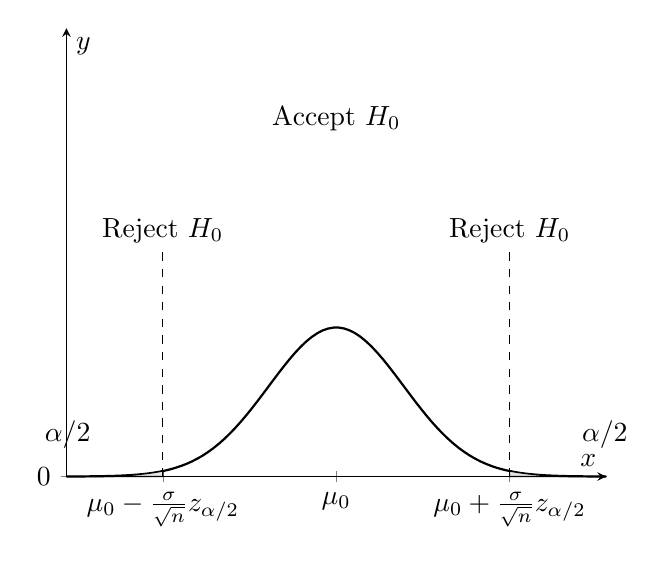
\begin{tikzpicture}
        \begin{axis}[
            axis lines=middle,
            xlabel=$x$,
            ylabel=$y$,
            xmin=-4,
            xmax=4,
            ymin=0,
            ymax=1.2,
            xtick={-2.571, 0, 2.571},
            xticklabels={$\mu_0-\frac{\sigma}{\sqrt{n}}z_{\alpha/2}$, $\mu_0$, $\mu_0+\frac{\sigma}{\sqrt{n}}z_{\alpha/2}$},
            ytick={0},
            yticklabels={0},
            axis x line=bottom,
            axis y line=left,
            domain=-4:4,
            samples=100,
            enlargelimits=false,
            clip=false
        ]
        
        \addplot[thick, black] {exp(-x^2/2)/sqrt(2*pi)};
        
        \addplot[fill=gray!20, domain=-4:-2.571] {exp(-x^2/2)/sqrt(2*pi)} \closedcycle;
        \node[above left] at (-3.5, 0.05) {$\alpha/2$};
        
        \addplot[fill=gray!20, domain=2.571:4] {exp(-x^2/2)/sqrt(2*pi)} \closedcycle;
        \node[above right] at (3.5, 0.05) {$\alpha/2$};
        
        \node[above] at (-2.571, 0.6) {Reject $H_0$};
        \node[above] at (0, 0.9) {Accept $H_0$};
        \node[above] at (2.571, 0.6) {Reject $H_0$};
        
        % Add vertical lines to emphasize the rejection regions
        \draw[dashed] (-2.571, 0) -- (-2.571, 0.6);
        \draw[dashed] (2.571, 0) -- (2.571, 0.6);
        \end{axis}
        \end{tikzpicture}
    \end{center}
    in other words it is 
    $$ \bar{x} \geq \mu_0 + z_{\alpha/2} \frac{\sigma}{\sqrt{n}} \quad \text{or} \quad \bar{x} \leq \mu_0 - z_{\alpha/2} \frac{\sigma}{\sqrt{n}}$$
    For a 1-sided test, alternative hypothesis is $H_1: \theta > \theta_0$ the likelihood ratio technique leads to a 1-sided test with critical region
    $$ \bar{x} \geq \mu_0 + z_{\alpha} \frac{\sigma}{\sqrt{n}}$$
    For a 1-sided test, alternative hypothesis is $H_1: \theta < \theta_0$ the likelihood ratio technique leads to a 1-sided test with critical region
    $$ \bar{x} \leq \mu_0 - z_{\alpha} \frac{\sigma}{\sqrt{n}}$$
\end{definition}
\begin{definition}[Steps to outline a Test of Hypothesis]
    Steps: 
    \begin{enumerate}
        \item Formulate $H_0$ and $H_1$ and choose the significance level $\alpha$.
        \item Using the sampling distribution of an appropriate test statisc determine a critica region of size $\alpha$ 
        \item Determine the value of the test statistic from the sample data
        \item Check whether the value of the test statistic falls into the critical reigion and accordingly, reject the null hypothesis or reserve judgement
    \end{enumerate}
\end{definition}
\begin{definition}[P value]
    Corresponding to an observed value of a test statistic, the P-value is the lowest level of significance at which the null hypothesis could be rejected.\\
    With this approach we can ajust the steps of a test of hypothesis as follows:
    \begin{enumerate}
        \item Formulate $H_0$ and $H_1$ and choose the significance level $\alpha$.
        \item Specify the test statistic 
        \item Determine the value of the test statistic and the corresponding P-value from the sample data
        \item Check whether the P-value is less than or equal to $\alpha$ and accordingly, reject the null hypothesis or reserve judgement
    \end{enumerate}
\end{definition}
\begin{definition}[Test concerning Means]
    For means we take our test statistic to be 
    $$ z = \frac{\bar{x} - \mu_0}{\sigma/\sqrt{n}}$$
    We can say this corresponding to a normal distribution, and thus we can use the normal distribution to find the critical region.
\end{definition}
\begin{definition}[Test concerning Difference of Means]
    For difference of means we take our test statistic to be 
    $$ z = \frac{\bar{x_1} - \bar{x_2} -(\mu_1 - \mu_2)}{\sqrt{\frac{\sigma_1^2}{n_1} + \frac{\sigma_2^2}{n_2}}}$$
    When we have unknown variances we can use the pooled variance
\end{definition}
\begin{definition}[Test concerning Variance]
    For variance we take our test statistic to be 
    $$ \chi^2 = \frac{(n-1)s^2}{\sigma_0^2}$$
    Where our $\sigma_0^2$ is the hypothesized variance.
    We can say this corresponding to a chi-squared distribution, and thus we can use the chi-squared distribution to find the critical region.
\end{definition}


\end{document}